% 比奥萨伐尔定律

\subsection{结论}
\begin{equation}
\bvec B(\bvec r) = \frac{\mu_0}{4\pi} \oint \frac{I \dd{\bvec r'} \cross \uvec R}{R^2}
\end{equation}
\subsection{说明}
比奥萨伐尔定律是一个\bb{定律}, 即电磁学的基本假设之一,所以以下并不是推导,而是解释公式的意义.

一个粗细忽略不计的电流回路中有电流 $I$, 如何确定该回路在空间中任意一点所产生的磁场呢? 由于磁场与电场一样可以叠加,我们可以把回路划分成极小的线段,分别计算每个小线段在某点产生的磁场,然后求和.当这些小线段的长度趋近于零,求和就变成了积分.那如何计算一小段长度为 $\dd{l}$ 的电流(电流元)产生的磁场呢? 如图(%图未完成,
 $\dd{l}$ 存在正方向,与 $\bvec R$ 的夹角为 $\theta$ ),为了表示电流的方向,我们先把 $\dd{l}$ 变为矢量 $\dd{\bvec l}$, 方向为电流的正方向(当 $I > 0$ 时,电流方向与 $\dd{\bvec l}$ 相同, $I < 0$ 时相反).现在我们要求空间中任意一点 $\bvec r$ (把这点叫做场点)的磁场,设电流元的位置为 $\bvec r$ (把这点叫做原点),且设
\begin{equation}
\bvec R = \bvec r - \bvec r'
\end{equation}
首先,磁场大小正比于 $I$, 这是合理的,因为如果把两小段电流元重叠放在一起,那么根据叠加原理,任何地方的磁场都会增加一倍.其次,与点电荷的电场(库仑定律)类似,场强与距离的平方成反比.最后,由于电流有特定的方向,磁场不再具有球对称,但具有柱对称.磁场大小正比于 $\abs{\dd{\bvec l} \cross \bvec R} = R \dd{l} \sin\theta $ (磁场方向垂直于 $\dd{\bvec l}$ 和 $\bvec R$ 所在平面,符合右手定则,见矢量的叉乘\upref{Cross}).这说明,在 $I$ 和 $R$ 不变时,垂直于电流元的点( $\theta  = \pi /2$ )具有最大场强,与其共线的点( $\theta  = 0$ )场强为零.

要注意的是,虽然我们是对单独一个 $I\dd{\bvec l}$ 分析,但稳定的电流元在现实中并不存在.因为线电流必须组成环路,否则在两个端点处就会分别积累大量的异号电荷(见电流的连续性),从而产生变化的电场及磁场,而在静态电磁场问题中,我们要求净电荷和电流的分布不随时间改变.所以在利用比奥萨伐尔公式时,必须要以对整个闭合回路积分 (无穷长直导线或者螺线管等理想问题除外%未完成;链接
若给所有的小电流源编号为 $I\dd{\bvec l_i}$, 令第 $i$ 个电流源的起点为 $\bvec r'_i$, $\bvec R_i = \bvec r - \bvec r'_i$.把所有电场矢量相加,变为
\begin{equation}
\bvec B (\bvec r) = \frac{\mu_0}{4\pi} \sum\limits_i \frac{I \dd{\bvec l_i} \cross \bvec R_i}{R_i^2}
\end{equation}
当电流元无穷短,数量无穷多的时候,上式写为积分的形式,且由于第 $i$ 个电流元的终点就是第 $i+1$ 个电流元的起点, $\dd{\bvec l_i} = \bvec r'_{i + 1} - \bvec r'_i = \dd{\bvec r'}$, 矢量积分写为
\begin{equation}\label{BioSav_eq4}
\bvec B (\bvec r) = \frac{\mu_0}{4\pi} \oint \frac{I\dd{\bvec r'} \cross \uvec R}{R^2}
\end{equation}
注意 $\bvec R$ 是场点 $\bvec r$ 和源点 $\bvec r'$ 的函数,积分时把 $\bvec r$ 视为常数而对 $\bvec r'$ 积分.为了使公式更明确,在难度较大的电磁学教材中把上式直接记为
\begin{equation}\label{BioSav_eq1}
\bvec B(\bvec r) = \frac{\mu_0}{4\pi} \oint \frac{I \dd{\bvec r'} \cross (\bvec r - \bvec r')}{\abs{\bvec r - \bvec r'}^3}
\end{equation}

\begin{figure}[ht]
\centering
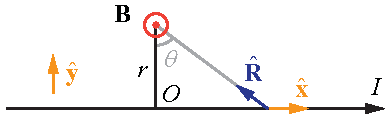
\includegraphics[width=6.4cm]{./figures/BioSav1.pdf}
\caption{无限长直导线的电场} \label{BioSav_fig1}
\end{figure}

\begin{exam}{无限长直导线的电场}\label{BioSav_exe1}
如\autoref{BioSav_fig1}, 令导线与 $x$ 轴重合, 并使原点到场点的距离最近, 有 $x = r\tan\theta$, 微分得 $\abs{\dd{\bvec r'}} = \dd{x} = r\sec^2\theta\dd{\theta}$, 另有 $\uvec x\cross\uvec R = \uvec z\sin(\theta + \pi/2) = \uvec z\cos\theta $, $R = r/\cos\theta$. 代入\autoref{BioSav_eq4} 得
\begin{equation}
\bvec B = \frac{\mu_0}{4\pi} I \uvec z\int_{-\pi/2}^{\pi/2} \frac{(r \sec^2\theta \dd{\theta}) \cos\theta}{r^2/\cos\theta^2}
= \frac{\mu_0}{4\pi} \frac Ir \uvec z\int_{-\pi/2}^{\pi/2} \cos\theta \dd{\theta}
= \frac{\mu_0}{2\pi} \frac Ir\uvec z
\end{equation}
可见磁场大小与距离 $r$ 成反比, 总是垂直于导线, 且方向符合右手定则.
\end{exam}

\subsection{矢量积分的计算方法}
比奥萨伐尔定律的积分中含有矢量微元的叉乘,看起来和普通的矢量积分不同,但是在常见的简单问题中,可以从几何理解上直接转换为标量的积分(见无限长直导线的磁场和环形电流轴线的磁场).如果是更一般的问题,则可以把叉乘分解成 3 个分量,然后变为 6 个标量积分
\begin{equation}\ali{
\dd{\bvec r'} \cross \bvec R &=
\begin{vmatrix}
\uvec x & \uvec y & \uvec z\\
\dd{x'} & \dd{y'} & \dd{z'}\\
x - x' & y - y' & z - z'
\end{vmatrix}\\
&= \uvec x [(z - z')\dd{y'} - (y - y')\dd{z'}] + \uvec y [\dots] + \uvec z[\dots]
}\end{equation}

\begin{equation}\ali{
\bvec B(\bvec r) &= \frac{\mu_0}{4\pi} \oint \frac{I\dd{\bvec r'} \cross \uvec R}{R^2}
= \frac{\mu_0 I}{4\pi} \oint \frac{\dd{\bvec r'} \cross \bvec R}{R^3} \\
& = \uvec x \frac{\mu_0 I}{4\pi} \qty[ \oint \frac{1}{R^3} (z - z') \dd{y'} - \oint \frac{1}{R^3} (y - y') \dd{z'} ] + \uvec y[\dots] + \uvec z[\dots]
}\end{equation}

\subsection{电流密度的形式}
假设电流的空间分布是连续变化的而不能看成一条截面不计曲线,我们需要用电流密度 $\bvec J$ 来表示空间的电流分布.现在考虑一个粗细不能忽略的环路, $\bvec r'$ 处的截面积为 $A$ (取截面时应垂直于电流),通过截面的电流为 $I = A\bvec J$, 所以电流元变为 $I \dd{\bvec l} = \bvec JA \dd{l} = \bvec J \vdot \dd{V}$ (根据定义, $\dd{\bvec l}$ 与 $\bvec J$ 的正方向相同), $\dd{V}$ 是电流元的体积.于是比奥萨伐尔定律的环路积分变为体积分
\begin{equation}
\bvec B(\bvec r) = \frac{\mu_0}{4\pi} \int \frac{\bvec J(\bvec r') \cross \uvec R}{R^2}\dd{V'}
\end{equation}
注意积分内的电流密度是关于源点的函数而不是场点的函数.理论上,体积分应该在导线内部进行,然而导线外部电流密度为零,故积分可以对全空间进行.类比式\autoref{BioSav_eq1}, 更明确的写法是
\begin{equation}
\bvec B(\bvec r) = \frac{\mu_0}{4\pi} \int \frac{\bvec J(\bvec r') \cross (\bvec r - \bvec r')}{\abs{\bvec r - \bvec r'}^3} \dd{V'}
\end{equation}
积分时 $\bvec r$ 视为常数.

